\documentclass[aspectratio=169,12pt,t]{beamer}

% --- Theme: Metropolis (modern, clean) ---
\usetheme[progressbar=frametitle,numbering=fraction,block=fill]{metropolis}

% --- Fira Sans font (install texlive-fonts-extra if missing) ---
\IfFileExists{FiraSans.sty}{\usepackage[sfdefault]{FiraSans}}{}

% --- Light background with warm accent ---
\definecolor{mDarkTeal}{RGB}{35,55,59}
\definecolor{mLightBrown}{RGB}{235,228,216}
\definecolor{mAccent}{RGB}{140,70,20}

\setbeamercolor{normal text}{fg=mDarkTeal,bg=white}
\setbeamercolor{alerted text}{fg=mAccent}
\setbeamercolor{frametitle}{bg=mDarkTeal,fg=white}
\setbeamercolor{progress bar}{fg=mAccent,bg=mLightBrown}
\setbeamercolor{title separator}{fg=mAccent}
\setbeamercolor{progress bar in head/foot}{fg=mAccent,bg=mLightBrown}
\setbeamercolor{progress bar in section page}{fg=mAccent,bg=mLightBrown}

% --- Packages ---
\usepackage[utf8]{inputenc}
\usepackage{amsmath,amssymb,amsthm}
\usepackage{mathrsfs}
\usepackage{tikz}
\usetikzlibrary{arrows.meta,positioning,calc,decorations.pathreplacing,shapes,patterns}
\usepackage{pgfplots}
\pgfplotsset{compat=1.18}

% --- Semi-transparent white highlight for text on top of background images ---
\usepackage[most]{tcolorbox}

% Inline highlight: \hl{short text}
\newtcbox{\hl}{%
  nobeforeafter, tcbox raise base,
  colback=white, opacityback=0.6,
  colframe=white, opacityframe=0,
  sharp corners, boxsep=2pt, left=3pt, right=3pt, top=2pt, bottom=2pt%
}

% Block highlight: \begin{hlbox} ... \end{hlbox}  (multi-line, paragraphs, itemize)
\newtcolorbox{hlbox}[1][]{%
  enhanced, breakable,
  colback=white, opacityback=0.6,
  colframe=white, opacityframe=0,
  boxsep=3pt, left=6pt, right=6pt, top=4pt, bottom=4pt,
  sharp corners,
  {#1}%
}

% --- Custom colors for content types ---
\definecolor{defcolor}{RGB}{25,85,120}
\definecolor{thmcolor}{RGB}{140,35,35}
\definecolor{proofcolor}{RGB}{35,100,50}
\definecolor{excolor}{RGB}{140,75,10}
\definecolor{remcolor}{RGB}{90,90,90}

% --- Beamer blocks for mathematical content types (semi-transparent) ---
\tcbset{hlblockbase/.style={
  enhanced, breakable,
  coltitle=white, fonttitle=\bfseries,
  opacitybacktitle=0.8, opacityback=0.6,
  opacityframe=0,
  sharp corners,
  boxsep=1pt, left=5pt, right=5pt, top=2pt, bottom=2pt,
  toptitle=1pt, bottomtitle=1pt
}}

\newtcolorbox{defblock}[1]{hlblockbase, title={#1},
  colbacktitle=defcolor, colback=defcolor!15, colframe=defcolor}
\newtcolorbox{thmblock}[1]{hlblockbase, title={#1},
  colbacktitle=thmcolor, colback=thmcolor!15, colframe=thmcolor}
\newtcolorbox{proofblock}[1]{hlblockbase, title={#1},
  colbacktitle=proofcolor, colback=proofcolor!15, colframe=proofcolor}
\newtcolorbox{exblock}[1]{hlblockbase, title={#1},
  colbacktitle=excolor, colback=excolor!15, colframe=excolor}
\newtcolorbox{remblock}[1]{hlblockbase, title={#1},
  colbacktitle=remcolor, colback=remcolor!15, colframe=remcolor}

% --- Metadata ---
\title{Chapter 3: Numerical Sequences and Series}
\subtitle{Section: Series}
\author{Based on Walter Rudin's \emph{Principles of Mathematical Analysis}}
\date{}

\begin{document}

% =============================================================================
% TITLE AND OUTLINE
% =============================================================================
{
\usebackgroundtemplate{%
  
\includegraphics[width=\paperwidth,height=\paperheight,keepaspectratio=false]{chapter_03_bg_00.png}%
}
\begin{frame}[plain]
  \titlepage
  \note{
    Welcome back to Chapter 3 of Principles of Mathematical Analysis.
    So far we have built up a careful theory of numerical sequences:
    what it means for a sequence to converge, Cauchy sequences,
    upper and lower limits, and the five special limits collected in
    Theorem 3.20. In this section we make the long-awaited turn to
    infinite series. We will define what it means to add infinitely
    many complex numbers, restate the Cauchy criterion in this new
    language, observe that the terms of a convergent series must
    tend to zero, and prove our first real convergence test, the
    comparison test. From here on, all sequences and series under
    consideration are complex-valued unless we explicitly say
    otherwise.
  }
\end{frame}
}

{
\usebackgroundtemplate{%
  
\includegraphics[width=\paperwidth,height=\paperheight,keepaspectratio=false]{chapter_03_bg_01.png}%
}
\begin{frame}[c]{Outline}
  \begin{center}
    \tableofcontents
  \end{center}
  \note{
    Here is the plan for this section. We start with motivation:
    why infinite sums show up everywhere and what could go wrong if
    we are not careful. We then write down Definition 3.21, which
    turns an infinite sum into a sequence of partial sums. With that
    in hand, the Cauchy criterion for sequences, Theorem 3.11,
    translates directly into Theorem 3.22, the Cauchy criterion for
    series. A one-line consequence is Theorem 3.23: the terms of a
    convergent series must vanish. Theorem 3.24 specialises to
    nonnegative-term series, where convergence is the same as
    boundedness of the partial sums. We finish with the comparison
    test, Theorem 3.25, our first practical convergence test.
  }
\end{frame}

% =============================================================================
% MOTIVATION
% =============================================================================
\section{Motivation}

% --- Build 1/4 ---
\begin{frame}{From Sequences to Series}
  \begin{hlbox}
    \begin{itemize}
      \item So far: theory of \alert{sequences} $\{a_n\}$
    \end{itemize}
  \end{hlbox}

  \note{
    Up to this point in the chapter, the basic object has been a
    sequence: an ordered list of numbers indexed by 1, 2, 3, and so
    on. We learned what it means for such a list to converge, what
    Cauchy sequences are, and how to compute several standard
    limits.
  }
\end{frame}

% --- Build 2/4 ---
\begin{frame}{From Sequences to Series}
  \begin{hlbox}
    \begin{itemize}
      \item So far: theory of \alert{sequences} $\{a_n\}$
      \item Yet many natural quantities are \emph{infinite sums}:
        $\;1 + \tfrac{1}{2} + \tfrac{1}{4} + \cdots,\quad 1 - \tfrac{1}{3} + \tfrac{1}{5} - \cdots$
    \end{itemize}
  \end{hlbox}

  \note{
    But many of the most useful quantities in mathematics are not
    single numbers, and not just sequences either: they are infinite
    sums. The first expression on the slide is the geometric series
    one plus one half plus one quarter and so on, which should equal
    2. The second is the Leibniz alternating series for pi over 4.
    These objects have been around since the dawn of calculus.
  }
\end{frame}

% --- Build 3/4 ---
\begin{frame}{From Sequences to Series}
  \begin{hlbox}
    \begin{itemize}
      \item So far: theory of \alert{sequences} $\{a_n\}$
      \item Yet many natural quantities are \emph{infinite sums}:
        $\;1 + \tfrac{1}{2} + \tfrac{1}{4} + \cdots,\quad 1 - \tfrac{1}{3} + \tfrac{1}{5} - \cdots$
      \item \alert{Problem:} we cannot literally add \emph{infinitely many} numbers
    \end{itemize}
  \end{hlbox}

  \note{
    There is a basic problem. The plus sign is a binary operation
    defined for two numbers at a time. Adding finitely many numbers
    extends without trouble, but adding infinitely many numbers is
    not a single operation we can perform. We need a precise
    definition of what an infinite sum even means.
  }
\end{frame}

% --- Build 4/4 ---
\begin{frame}{From Sequences to Series}
  \begin{hlbox}
    \begin{itemize}
      \item So far: theory of \alert{sequences} $\{a_n\}$
      \item Yet many natural quantities are \emph{infinite sums}:
        $\;1 + \tfrac{1}{2} + \tfrac{1}{4} + \cdots,\quad 1 - \tfrac{1}{3} + \tfrac{1}{5} - \cdots$
      \item \alert{Problem:} we cannot literally add \emph{infinitely many} numbers
      \item \alert{Idea:} reduce to sequences via the \emph{partial sums} $s_n = a_1 + \cdots + a_n$
    \end{itemize}
  \end{hlbox}

  \note{
    The classical idea, going back to Cauchy, is to reduce the
    problem to one we already understand. Instead of asking for the
    infinite sum directly, we form the partial sums: "s" sub 1 is
    just "a" sub 1, "s" sub 2 is "a" sub 1 plus "a" sub 2, "s" sub
    3 is "a" sub 1 plus "a" sub 2 plus "a" sub 3, and so on. That
    gives a sequence of perfectly ordinary finite sums, and we ask
    whether this sequence converges. If it does, its limit is what
    we call the sum of the series. That is the definition we make
    precise next.
  }
\end{frame}
}

{
\usebackgroundtemplate{%
  
\includegraphics[width=\paperwidth,height=\paperheight,keepaspectratio=false]{chapter_03_bg_02.png}%
}
% =============================================================================
% SERIES AND PARTIAL SUMS
% =============================================================================
\section{Series and Partial Sums}

% --- Standing convention ---
\begin{frame}{A Standing Convention for the Rest of the Chapter}
  \begin{remblock}{Convention}
    In the remainder of Chapter 3, all sequences and series are
    \alert{complex-valued} unless explicitly stated otherwise.
  \end{remblock}

  \vspace{0.6em}
  \begin{hlbox}
    Extensions to $\mathbb{R}^k$-valued series are treated in
    Exercise 15.
  \end{hlbox}

  \note{
    Before we write the definition, one piece of bookkeeping. From
    this section onward, every sequence and every series in
    Chapter 3 is allowed to be complex-valued. Whatever we prove
    about complex series automatically covers the real case as a
    special case. Extensions to vector-valued series in real "k"
    dimensional space are pushed to Exercise 15, since they require
    nothing essentially new. Now to the definition.
  }
\end{frame}

% --- Definition 3.21: finite sum notation ---
\begin{frame}{Definition 3.21: Finite Sum Notation}
  \begin{defblock}{Finite sums: the $\Sigma$ symbol}
    Given a sequence $\{a_n\}$ and integers $p \leq q$,
    \[
      \sum_{n=p}^{q} a_n \;=\; a_p + a_{p+1} + \cdots + a_q .
    \]
  \end{defblock}

  \vspace{0.6em}
  \begin{hlbox}
    Capital sigma, $\Sigma$, is just compact notation for a finite
    sum --- nothing infinite yet.
  \end{hlbox}

  \note{
    Definition 3.21 opens with a piece of notation we will lean on
    constantly. The capital sigma symbol shown on the slide bundles
    a finite sum of consecutive terms into one compact expression:
    a starting index "p" sits below, an ending index "q" sits above,
    and the dummy index "n" runs over every integer in between,
    picking out the term "a" sub "n" each time and adding them
    together.

    Two points are worth stressing. First, the notation is purely
    cosmetic: it stands for an ordinary finite sum and nothing
    more. Second, that finite-sum interpretation is exactly why it
    matters. Once we let "q" run off to infinity in a moment, the
    same symbol will pivot from short-hand into the central object
    of the section, the infinite series.
  }
\end{frame}

% --- Definition 3.21: partial sums ---
\begin{frame}{Definition 3.21: Partial Sums and the Series Symbol}
  \begin{defblock}{Partial sums and infinite series}
    With each sequence $\{a_n\}$ we associate the sequence of
    \alert{partial sums}
    \[
      s_n \;=\; \sum_{k=1}^{n} a_k \;=\; a_1 + a_2 + \cdots + a_n .
    \]
    The symbolic expression
    \begin{equation*}
      a_1 + a_2 + a_3 + \cdots \qquad\text{or, more concisely,}\qquad
      \sum_{n=1}^{\infty} a_n \tag{4}
    \end{equation*}
    is called an \emph{infinite series}, or just a \emph{series}.
  \end{defblock}

  \note{
    Now the central definition. Starting from a sequence "a" sub
    "n", we manufacture a brand-new sequence by accumulating the
    terms one at a time. The "n" th partial sum, written "s" sub
    "n" on the slide, is just the finite sum of the first "n"
    terms. Each "s" sub "n" is a perfectly ordinary finite sum;
    what is new is that we view them collectively, as their own
    sequence.

    Then, in the second display, we introduce the symbol we will
    actually use for the rest of the chapter: capital sigma with
    "n" running from 1 to infinity. The crucial point is what this
    symbol does not yet mean. At this stage it is a symbol, not a
    number. It carries no value until we ask whether the partial
    sums it stands for actually converge. Giving the symbol a
    numerical meaning is the job of the next slide.
  }
\end{frame}

% --- Definition 3.21: convergence ---
\begin{frame}{Definition 3.21: Convergence and the Sum}
  \begin{defblock}{Convergence, divergence, sum}
    If the partial sums $\{s_n\}$ converge to $s$, the series
    \alert{converges} and we write
    \[
      \sum_{n=1}^{\infty} a_n \;=\; s .
    \]
    The number $s$ is the \emph{sum of the series}. \\[0.2em]
    If $\{s_n\}$ diverges, the series \alert{diverges}.
  \end{defblock}

  \vspace{0.4em}
  \begin{remblock}{Crucial caveat}
    $s$ is the \alert{limit of a sequence of sums}, not a sum
    performed in one step.
  \end{remblock}

  \note{
    Here is where the symbol acquires a meaning. If the sequence of
    partial sums "s" sub "n" converges to some number "s", we say
    the series converges, and we use the very same sigma notation to
    denote the limit "s". This number "s" is called the sum of the
    series. If the partial sums fail to converge, the series is said
    to diverge.

    The gray block underlines a point that confuses every student
    sooner or later: the sum of an infinite series is not obtained
    by addition. There is no last term to add. It is a limit of a
    sequence of finite sums. The same sigma symbol is doing double
    duty: on the left it denotes the formal series, on the right it
    denotes its limit, when that limit exists.
  }
\end{frame}

% --- Definition 3.21: variations ---
\begin{frame}{Definition 3.21: Notational Variations}
  \begin{remblock}{Two notational shortcuts}
    \begin{itemize}
      \item Sometimes we start at $n = 0$:
        $\;\displaystyle\sum_{n=0}^{\infty} a_n$.
      \item When the starting index does not matter, we just write
        $\Sigma\, a_n$.
    \end{itemize}
  \end{remblock}

  \vspace{0.5em}
  \begin{hlbox}
    \textbf{Sequences and series are interchangeable:}\\[0.2em]
    Set $a_1 = s_1,\; a_n = s_n - s_{n-1}\;(n > 1)$ to go back from
    a sequence $\{s_n\}$ to its generating series.
  \end{hlbox}

  \note{
    Two quick conventions, both shown on the slide. Some series
    naturally start at index zero rather than one, which is what
    the first bullet records; the choice is cosmetic and we will
    switch between them freely. The second bullet says that when
    the starting index plays no role in an argument, we simply
    write capital sigma "a" sub "n" with no limits attached.

    The highlighted box at the bottom is the more substantive
    point. Sequences and series are really two views of the same
    data. Going one way, the partial sums of a series form a
    sequence by definition. Going the other way is just as easy:
    given any sequence, take the first term, and let each later
    term record the increment from one entry to the next; then the
    partial sums of those increments recover the original sequence
    exactly. So every result about sequences can be reread as a
    result about series, and vice versa. Both languages survive in
    the literature because each makes certain ideas easier to see
    than the other.
  }
\end{frame}

% --- Concrete example: geometric series 1 + 1/2 + 1/4 + ... ---
\begin{frame}{Example: The Partial Sums of $1 + \tfrac{1}{2} + \tfrac{1}{4} + \cdots$}
  \begin{center}
  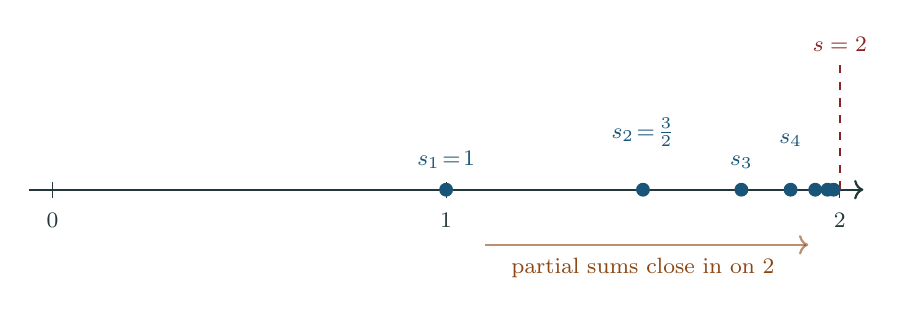
\begin{tikzpicture}[scale=1.0]
    % number line
    \draw[->, thick, mDarkTeal] (-0.3, 0) -- (10.3, 0);
    % ticks at 0, 1, 2
    \foreach \x/\lbl in {0/0, 5/1, 10/2} {
      \draw[mDarkTeal] (\x, -0.1) -- (\x, 0.1);
      \node[mDarkTeal, below=2pt] at (\x, -0.1) {\footnotesize $\lbl$};
    }
    % the limit at 2
    \draw[thick, thmcolor, dashed] (10, 0) -- (10, 1.6);
    \node[thmcolor] at (10, 1.85) {\footnotesize $s = 2$};
    % partial sums s_1 = 1, s_2 = 1.5, s_3 = 1.75, s_4 = 1.875, s_5 = 1.9375, s_6 = 1.96875
    \fill[defcolor] (5.0, 0) circle (2.5pt) node[above=4pt]{\footnotesize $s_1\!=\!1$};
    \fill[defcolor] (7.5, 0) circle (2.5pt) node[above=12pt]{\footnotesize $s_2\!=\!\tfrac{3}{2}$};
    \fill[defcolor] (8.75, 0) circle (2.5pt) node[above=4pt]{\footnotesize $s_3$};
    \fill[defcolor] (9.375, 0) circle (2.5pt) node[above=12pt]{\footnotesize $s_4$};
    \fill[defcolor] (9.6875, 0) circle (2.5pt);
    \fill[defcolor] (9.84375, 0) circle (2.5pt);
    \fill[defcolor] (9.921875, 0) circle (2.5pt);
    % arrow showing approach
    \draw[->, thick, mAccent, opacity=0.6] (5.5, -0.7) -- (9.6, -0.7);
    \node[mAccent] at (7.5, -1.0) {\footnotesize partial sums close in on $2$};
  \end{tikzpicture}
  \end{center}

  \vspace{0.2em}
  \begin{center}
    \hl{Each $s_n$ shrinks the remaining gap by a factor of $2$.}
  \end{center}

  \note{
    A picture to make Definition 3.21 concrete. The slide shows the
    partial sums of the geometric series 1 plus one half plus one
    quarter plus one eighth and so on, plotted on the number line
    between 0 and 2. The dashed red line at 2 marks where these
    partial sums are heading.

    Reading the blue dots from the left, "s" sub 1 is 1, "s" sub 2
    is 3 halves, "s" sub 3 is 7 fourths, "s" sub 4 is 15 eighths,
    and so on. Each partial sum lands exactly halfway between the
    previous one and 2. The amber arrow underneath captures the
    motion: the partial sums march steadily to the right but never
    overshoot, closing in on 2. Since this sequence of partial sums
    converges to 2, Definition 3.21 says that the series converges
    and that its sum is 2. The infinite sum is meaningful exactly
    because the sequence of finite sums has a limit.
  }
\end{frame}
}

{
\usebackgroundtemplate{%
  
\includegraphics[width=\paperwidth,height=\paperheight,keepaspectratio=false]{chapter_03_bg_03.png}%
}
% =============================================================================
% CAUCHY CRITERION
% =============================================================================
\section{The Cauchy Criterion for Series}

% --- Restating the Cauchy criterion for series ---
\begin{frame}{Theorem 3.22: Cauchy Criterion for Series}
  \begin{thmblock}{Theorem 3.22}
    $\Sigma\, a_n$ converges \alert{if and only if} for every
    $\varepsilon > 0$ there is an integer $N$ such that
    \begin{equation*}
      \left|\sum_{k=n}^{m} a_k\right| \;\leq\; \varepsilon
      \qquad\text{whenever } m \geq n \geq N. \tag{6}
    \end{equation*}
  \end{thmblock}

  \vspace{0.4em}
  \begin{hlbox}
    \textbf{Idea:} apply the Cauchy criterion for \emph{sequences}
    (Theorem 3.11) to the partial sums $\{s_n\}$.
  \end{hlbox}

  \note{
    Theorem 3.22 is the Cauchy criterion translated into the
    language of series. Reading the displayed condition: for every
    positive epsilon there is an index "N" past which every block
    sum, that is every consecutive piece of the series taken from
    index "n" up to index "m", is at most epsilon in absolute
    value. The slogan version: every far-out chunk of the series
    is uniformly tiny.

    The reason this is such a powerful tool is in what it does not
    require. We can use it to prove convergence without ever
    knowing what the sum is. For almost every series we will meet
    after this section, there is no closed form for the sum; the
    Cauchy criterion is what lets us still say "yes, it converges"
    in those cases. The idea behind the proof, recorded in the
    highlighted box, is simply to apply the Cauchy criterion for
    sequences, Theorem 3.11, to the sequence of partial sums. The
    next slide makes that translation concrete.
  }
\end{frame}

% --- Why Theorem 3.22 follows from Theorem 3.11 ---
\begin{frame}{Why Theorem 3.22 Follows from Theorem 3.11}
  \begin{proofblock}{The translation in one identity}
    For $m \geq n \geq 1$,
    \[
      s_m - s_{n-1} \;=\; \sum_{k=n}^{m} a_k .
    \]
    So a block sum on the right is the \alert{difference of two
    partial sums}.
  \end{proofblock}

  \vspace{0.4em}
  \begin{hlbox}
    \textbf{Therefore:}
    $|\sum_{k=n}^{m} a_k| \leq \varepsilon$ for all $m \geq n \geq N$\\
    $\iff |s_m - s_{n-1}| \leq \varepsilon$ for all $m \geq n \geq N$\\
    $\iff \{s_n\}$ is Cauchy
    $\iff \{s_n\}$ converges (Theorem 3.11)\\
    $\iff \Sigma\, a_n$ converges.
  \end{hlbox}

  \note{
    The whole proof rests on one simple observation, sitting in the
    green proof block. Subtracting two partial sums collapses by
    telescoping: the shared terms cancel, and what is left is
    exactly the block sum running from index "n" through index
    "m". So a block sum of the original series is nothing other
    than a difference of partial sums in disguise.

    With that identity in hand, the highlighted box becomes a chain
    of equivalences. Bounding the block sum by epsilon is the same
    as bounding a difference of partial sums by epsilon. That bound,
    holding for all sufficiently large indices, is exactly the
    Cauchy condition on the sequence of partial sums. Theorem 3.11
    then says a Cauchy sequence converges, and converging partial
    sums is precisely how we defined a convergent series. So
    Theorem 3.22 is not really a new theorem at all. It is
    Theorem 3.11 reread in series language.
  }
\end{frame}
}

{
\usebackgroundtemplate{%
  
\includegraphics[width=\paperwidth,height=\paperheight,keepaspectratio=false]{chapter_03_bg_04.png}%
}
% =============================================================================
% TERMS MUST VANISH
% =============================================================================
\section{Vanishing of the Terms}

% --- Theorem 3.23: necessary condition ---
\begin{frame}{Theorem 3.23: A Necessary Condition for Convergence}
  \begin{thmblock}{Theorem 3.23}
    If $\Sigma\, a_n$ converges, then $\displaystyle\lim_{n \to \infty} a_n = 0$.
  \end{thmblock}

  \vspace{0.5em}
  \begin{proofblock}{Why: take $m = n$ in Theorem 3.22}
    With $m = n$, the block sum is just the single term $a_n$, so
    (6) becomes
    \[
      |a_n| \leq \varepsilon \qquad (n \geq N).
    \]
    Hence $a_n \to 0$. \quad $\Box$
  \end{proofblock}

  \note{
    Theorem 3.23 is a free corollary of the Cauchy criterion: if a
    series converges, its terms must tend to zero. The intuition is
    easy to feel. If the terms refused to shrink, every new term
    would knock the partial sum sideways by at least some fixed
    positive amount, and a sequence that keeps jumping by a fixed
    amount cannot settle down to a limit.

    The proof on the slide makes that intuition rigorous in one
    move. The Cauchy criterion gives us a uniform bound on every
    block sum from index "n" to index "m"; in particular we are
    free to take "m" equal to "n", in which case the block sum
    collapses to a single term, "a" sub "n". The criterion now says
    that single term is at most epsilon in absolute value once "n"
    is large enough, which is exactly the definition of "a" sub
    "n" tending to zero. So the terms going to zero is necessary
    for convergence. The next slide warns that it is not enough.
  }
\end{frame}

% --- Build 1/3: warning about the converse ---
\begin{frame}{Warning: The Converse Fails}
  \begin{remblock}{Theorem 3.23 is necessary, not sufficient}
    $a_n \to 0$ does \alert{not} imply $\Sigma\, a_n$ converges.
  \end{remblock}

  \note{
    A vital warning. Theorem 3.23 is a one-way street. Having the
    terms tend to zero is necessary for convergence, but it is not
    sufficient. There exist series whose terms shrink to zero and
    yet whose partial sums march off to infinity. Recognising this
    distinction will save you from many false proofs.
  }
\end{frame}

% --- Build 2/3: counterexample harmonic series ---
\begin{frame}{Warning: The Converse Fails}
  \begin{remblock}{Theorem 3.23 is necessary, not sufficient}
    $a_n \to 0$ does \alert{not} imply $\Sigma\, a_n$ converges.
  \end{remblock}

  \vspace{0.5em}
  \begin{exblock}{Standard counterexample: the harmonic series}
    The series
    \[
      \sum_{n=1}^{\infty} \frac{1}{n}
      \;=\; 1 + \tfrac{1}{2} + \tfrac{1}{3} + \tfrac{1}{4} + \cdots
    \]
    \alert{diverges}, even though $1/n \to 0$.
  \end{exblock}

  \note{
    The standard counterexample is the harmonic series: one plus
    one half plus one third plus one fourth and so on. The general
    term is 1 over "n", which clearly goes to zero. Nevertheless,
    the series diverges; its partial sums grow without bound. We
    will not prove the divergence here. It will follow as a special
    case of Theorem 3.28 in the next section, on series of
    nonnegative terms.
  }
\end{frame}

% --- Build 3/3: harmonic intuition ---
\begin{frame}{Warning: The Converse Fails}
  \begin{remblock}{Theorem 3.23 is necessary, not sufficient}
    $a_n \to 0$ does \alert{not} imply $\Sigma\, a_n$ converges.
  \end{remblock}

  \vspace{0.5em}
  \begin{exblock}{Standard counterexample: the harmonic series}
    The series
    \[
      \sum_{n=1}^{\infty} \frac{1}{n}
      \;=\; 1 + \tfrac{1}{2} + \tfrac{1}{3} + \tfrac{1}{4} + \cdots
    \]
    \alert{diverges}, even though $1/n \to 0$.
  \end{exblock}

  \vspace{0.4em}
  \begin{hlbox}
    The terms going to zero says \emph{nothing}
    about whether the sum is finite.
  \end{hlbox}

  \note{
    The moral, in the highlighted box, is worth repeating. Knowing
    the terms tend to zero by itself tells you nothing about
    whether the sum is finite. The terms can tend to zero too
    slowly to be summable. This is why we need genuine convergence
    tests, and why the rest of the chapter is devoted to building
    them.
  }
\end{frame}
}

{
\usebackgroundtemplate{%
  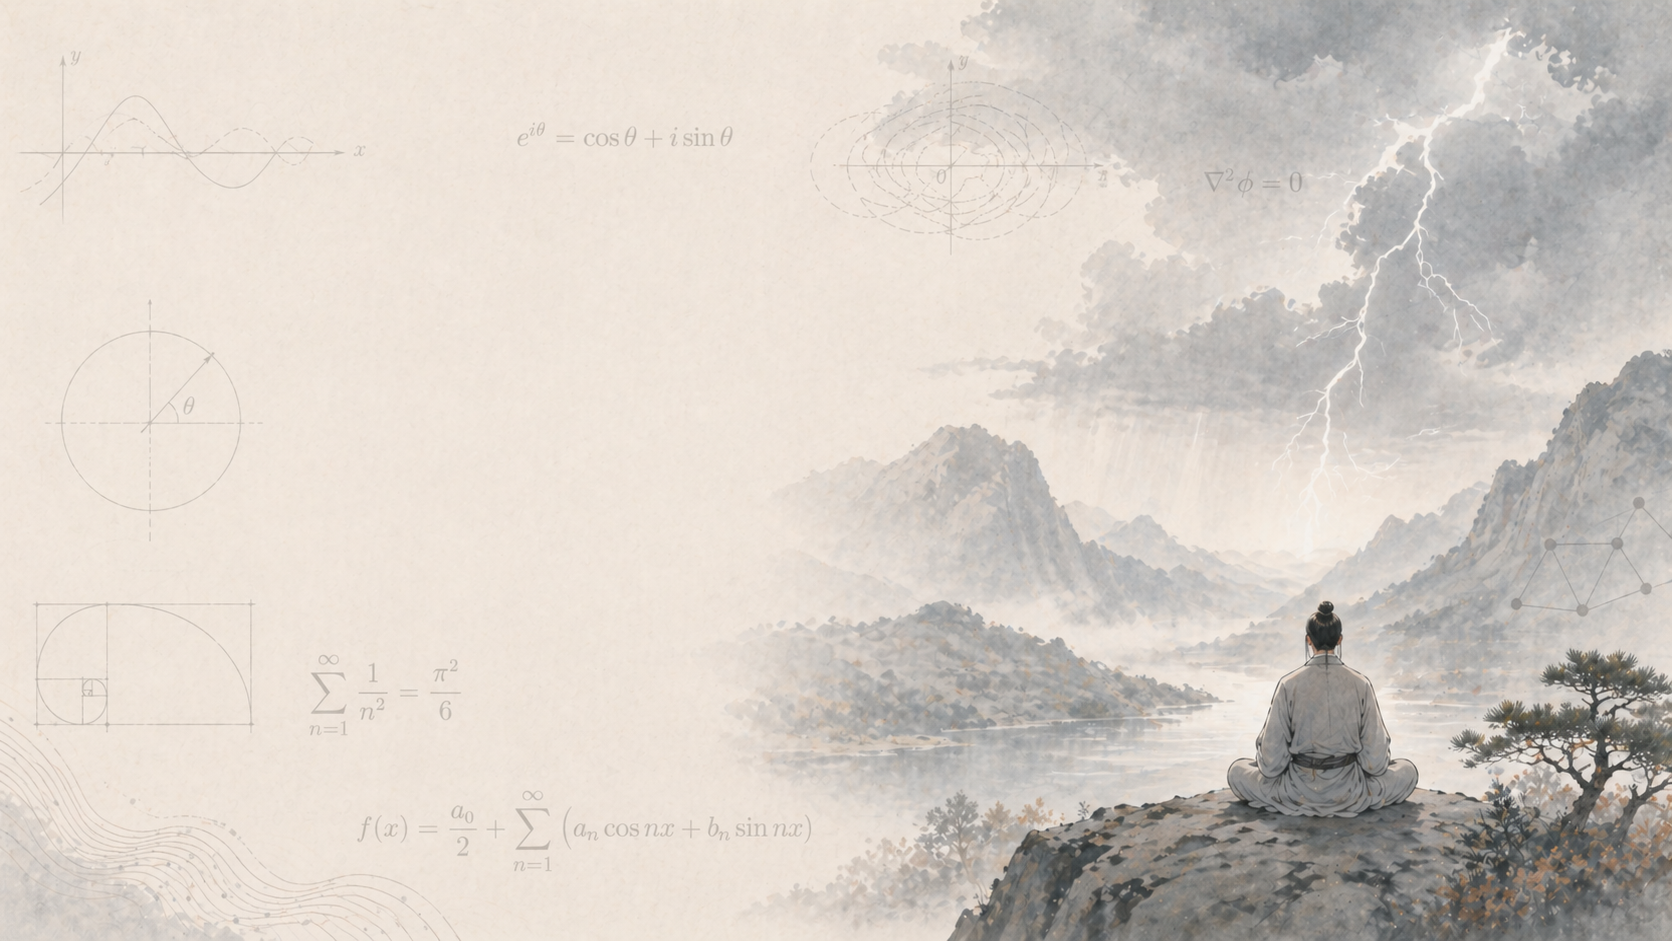
\includegraphics[width=\paperwidth,height=\paperheight,keepaspectratio=false]{chapter_03_bg_05.png}%
}
% =============================================================================
% NONNEGATIVE TERMS
% =============================================================================
\section{Series of Nonnegative Terms}

% --- Theorem 3.24 ---
\begin{frame}{Theorem 3.24: Nonnegative Series and Bounded Partial Sums}
  \begin{thmblock}{Theorem 3.24}
    A series of \alert{nonnegative real} terms converges
    \alert{if and only if} its partial sums form a bounded sequence.
  \end{thmblock}

  \vspace{0.5em}
  \begin{hlbox}
    \textbf{Idea:} when $a_n \geq 0$, the partial sums
    $s_n = a_1 + \cdots + a_n$ are \alert{monotonic}.
    \\[0.2em]
    Apply Theorem 3.14: monotonic + bounded $\Longrightarrow$
    convergent.
  \end{hlbox}

  \note{
    Theorem 3.24 is the series analogue of Theorem 3.14, the
    monotone convergence theorem for sequences. It is restricted to
    series of nonnegative real terms; the footnote in Rudin
    emphasises that nonnegative always refers to real numbers, since
    there is no useful ordering on the complex plane.

    The reason is in the highlighted box. When every term "a" sub
    "n" is nonnegative, adding the next term can only push the
    partial sum up or leave it where it is. So the partial sums
    form a monotonically nondecreasing sequence. A monotonic
    sequence converges if and only if it is bounded, by
    Theorem 3.14. Putting these together: convergence of the
    series is exactly boundedness of the partial sums.
  }
\end{frame}

% --- Visual: monotone staircase of partial sums ---
\begin{frame}{Picture: A Monotone Staircase of Partial Sums}
  \begin{center}
  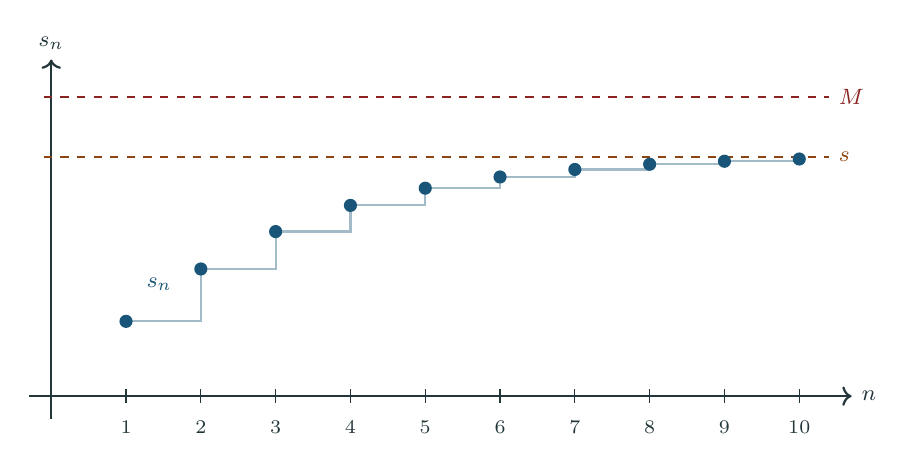
\begin{tikzpicture}[scale=0.95]
    % axes
    \draw[->, thick, mDarkTeal] (-0.3, 0) -- (10.7, 0) node[right]{\footnotesize $n$};
    \draw[->, thick, mDarkTeal] (0, -0.3) -- (0, 4.5) node[above]{\footnotesize $s_n$};
    % n-axis ticks at the integer indices n = 1, 2, ..., 10
    \foreach \n in {1,...,10} {
      \draw[mDarkTeal] (\n, -0.09) -- (\n, 0.09);
      \node[mDarkTeal, below=3pt] at (\n, -0.09) {\scriptsize \n};
    }
    % upper bound M
    \draw[thick, thmcolor, dashed] (-0.1, 4.0) -- (10.4, 4.0);
    \node[thmcolor, right] at (10.4, 4.0) {\footnotesize $M$};
    % limit s
    \draw[thick, mAccent, dashed] (-0.1, 3.2) -- (10.4, 3.2);
    \node[mAccent, right] at (10.4, 3.2) {\footnotesize $s$};
    % monotone partial sums approaching s from below
    \fill[defcolor] (1, 1.00) circle (2.5pt);
    \fill[defcolor] (2, 1.70) circle (2.5pt);
    \fill[defcolor] (3, 2.20) circle (2.5pt);
    \fill[defcolor] (4, 2.55) circle (2.5pt);
    \fill[defcolor] (5, 2.78) circle (2.5pt);
    \fill[defcolor] (6, 2.93) circle (2.5pt);
    \fill[defcolor] (7, 3.03) circle (2.5pt);
    \fill[defcolor] (8, 3.10) circle (2.5pt);
    \fill[defcolor] (9, 3.14) circle (2.5pt);
    \fill[defcolor] (10, 3.17) circle (2.5pt);
    % faint connecting steps to suggest the staircase
    \draw[defcolor, opacity=0.4, thick]
      (1,1.00) -- (2,1.00) -- (2,1.70) -- (3,1.70) -- (3,2.20)
      -- (4,2.20) -- (4,2.55) -- (5,2.55) -- (5,2.78)
      -- (6,2.78) -- (6,2.93) -- (7,2.93) -- (7,3.03)
      -- (8,3.03) -- (8,3.10) -- (9,3.10) -- (9,3.14)
      -- (10,3.14) -- (10,3.17);
    % label
    \node[defcolor, right=4pt] at (1, 1.5) {\footnotesize $s_n$};
  \end{tikzpicture}
  \end{center}

  \vspace{0.2em}
  \begin{center}
    \hl{\alert{Increasing} + \alert{bounded by $M$} $\Longrightarrow$ a finite limit $s \leq M$.}
  \end{center}

  \note{
    Here is the picture behind Theorem 3.24. The horizontal axis is
    the index "n", marked with ticks at the whole numbers 1 through
    10 to remind us that we are looking at a sequence, not a
    continuous function. The vertical axis is the value of the
    partial sum "s" sub "n". The blue dots are the partial sums of
    a nonnegative series, and the faint blue steps connecting them
    sketch the staircase shape.

    Because every term added is nonnegative, each blue dot sits at
    or above the previous one, so the staircase only rises or holds
    steady, never falling. The red dashed line is an upper bound
    "M": every dot stays below it. The monotone convergence theorem
    for sequences then guarantees a finite limit, marked by the
    amber dashed line at "s", and that limit sits at or below "M".
    If no such "M" existed, the staircase would simply keep
    climbing and the series would diverge to plus infinity. So for
    a nonnegative series, convergence is bounded staircase,
    divergence is unbounded staircase. Nothing in between.
  }
\end{frame}

% --- Why it matters ---
\begin{frame}{Why Theorem 3.24 Matters in Practice}
  \begin{hlbox}
    \textbf{Convergence reduces to a single quantitative question:}
    \begin{itemize}
      \item Is there a constant $M$ with
        $\;s_n = a_1 + a_2 + \cdots + a_n \leq M$ for all $n$?
      \item If yes, $\Sigma\, a_n$ converges (to some $s \leq M$).
      \item If no, $\Sigma\, a_n$ diverges to $+\infty$.
    \end{itemize}
  \end{hlbox}

  \vspace{0.4em}
  \begin{hlbox}
    This is what makes the \alert{comparison test} coming up so
    powerful.
  \end{hlbox}

  \note{
    Why is this so useful? Because, for nonnegative series, the
    qualitative question of convergence reduces to a single
    quantitative question: are the partial sums bounded above by
    some fixed constant "M". If yes, the series converges, and its
    sum is at most "M". If no, the partial sums are unbounded and,
    being nondecreasing, they march to plus infinity, so the
    series diverges.

    This reduction is what makes the comparison test, coming up in
    the next section, so effective. We no longer need to compute
    the sum exactly. We only need to bound the partial sums above
    by a series we already know is convergent. Hence the chapter's
    central strategy: catalogue a few known convergent series and
    use them as yardsticks.
  }
\end{frame}
}

{
\usebackgroundtemplate{%
  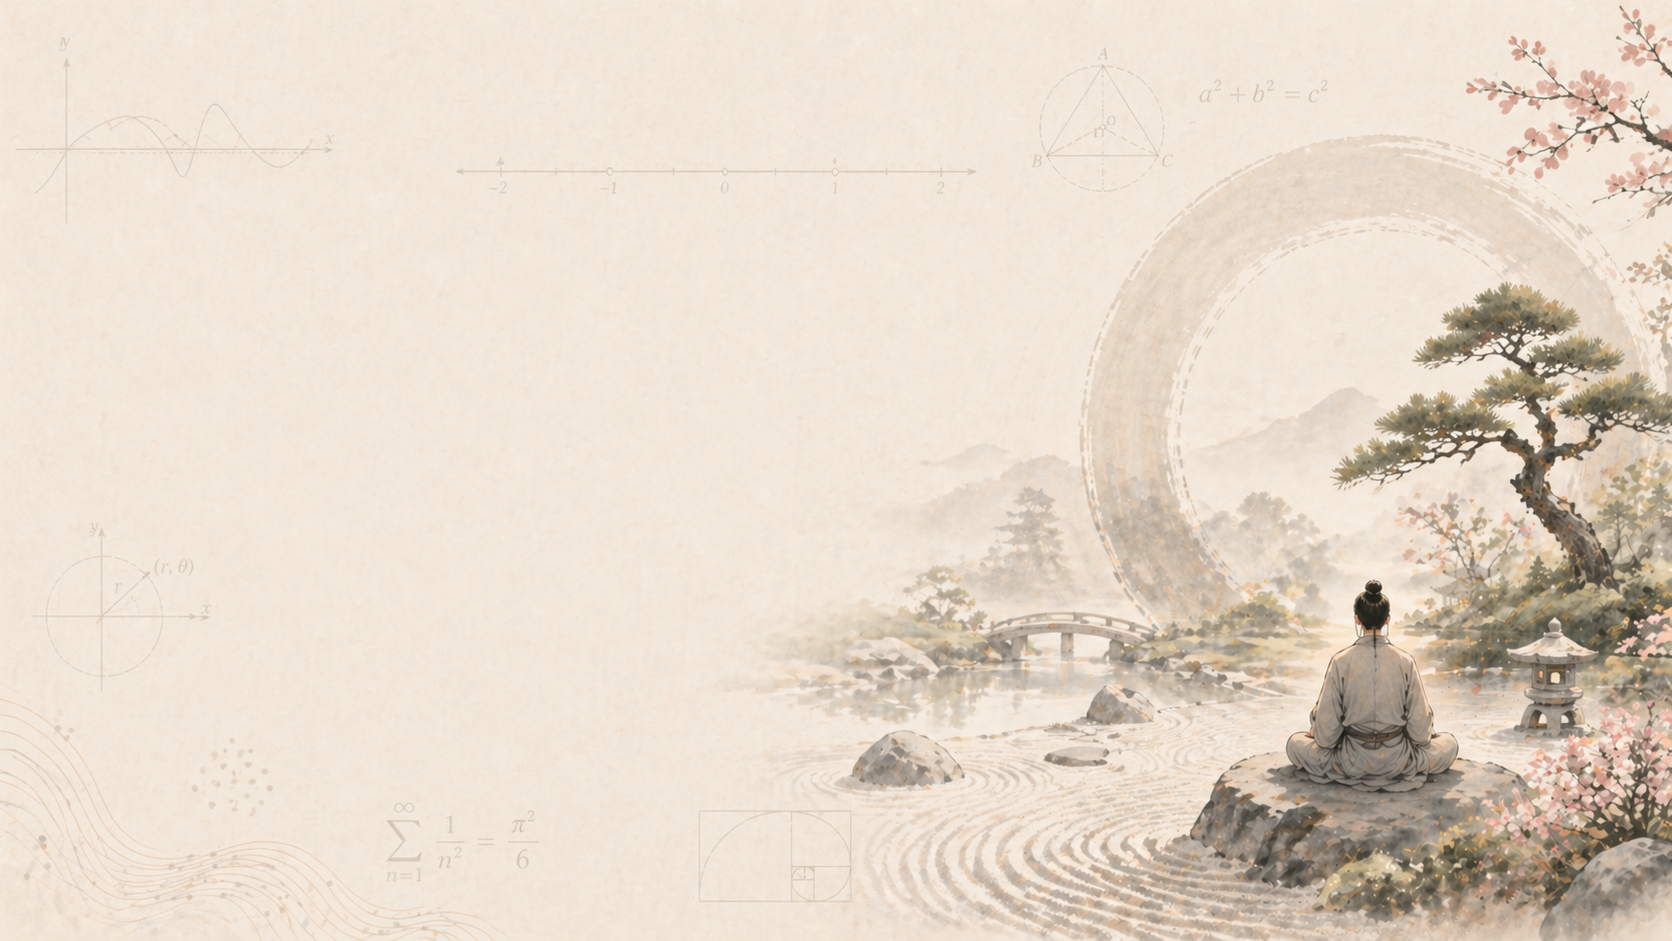
\includegraphics[width=\paperwidth,height=\paperheight,keepaspectratio=false]{chapter_03_bg_06.png}%
}
% =============================================================================
% THE COMPARISON TEST
% =============================================================================
\section{The Comparison Test}

% --- Theorem 3.25 statement ---
\begin{frame}{Theorem 3.25: The Comparison Test}
  \begin{thmblock}{Theorem 3.25 (Comparison test)}
    \begin{enumerate}
      \item[(a)] If $|a_n| \leq c_n$ for $n \geq N_0$ and
        $\Sigma\, c_n$ converges, then $\Sigma\, a_n$ converges.
      \item[(b)] If $a_n \geq d_n \geq 0$ for $n \geq N_0$ and
        $\Sigma\, d_n$ diverges, then $\Sigma\, a_n$ diverges.
    \end{enumerate}
  \end{thmblock}

  \vspace{0.4em}
  \begin{remblock}{Caveat}
    Part (b) applies only to series of \alert{nonnegative}
    terms $a_n$.
  \end{remblock}

  \note{
    Theorem 3.25 is the comparison test. It comes in two halves.

    Part "a" is the convergence half. If, past some fixed index "N"
    sub 0, the absolute value of "a" sub "n" is dominated by a
    nonnegative number "c" sub "n", and the dominating series of
    "c" sub "n" converges, then the original series of "a" sub "n"
    converges as well. The terms "a" sub "n" themselves can be
    complex.

    Part "b" is the divergence half. If the terms "a" sub "n" are
    nonnegative real numbers, and they dominate another nonnegative
    sequence "d" sub "n" whose series diverges, then the larger
    series of "a" sub "n" diverges too. The gray caveat is
    important: part "b" only makes sense for nonnegative real terms.
  }
\end{frame}

% --- Build 1/3: proof of (a) setup ---
\begin{frame}{Proof of Theorem 3.25 (a) --- Setup}
  \begin{proofblock}{Step 1: choose $N$ using Cauchy on $\Sigma\, c_n$}
    Since $\Sigma\, c_n$ converges, by Theorem 3.22, given
    $\varepsilon > 0$ there exists $N \geq N_0$ such that
    \[
      \sum_{k=n}^{m} c_k \;\leq\; \varepsilon
      \qquad\text{whenever } m \geq n \geq N .
    \]
  \end{proofblock}

  \note{
    On to the proof of part "a". Fix any positive epsilon. Since
    the dominating series "c" sub "n" is assumed to converge, the
    Cauchy criterion for series, Theorem 3.22, gives an index "N"
    past which every block sum of "c" sub "k" is at most epsilon.
    We pick "N" large enough that it is also at least "N" sub 0,
    so that the hypothesis on the original "a" sub "n" is in force
    for every index from "N" onward.
  }
\end{frame}

% --- Build 2/3: proof of (a) chain of inequalities ---
\begin{frame}{Proof of Theorem 3.25 (a) --- The Estimate}
  \begin{proofblock}{Step 2: triangle inequality + comparison}
    For $m \geq n \geq N$:
    \[
      \left|\sum_{k=n}^{m} a_k\right|
      \;\leq\; \sum_{k=n}^{m} |a_k|
      \;\leq\; \sum_{k=n}^{m} c_k
      \;\leq\; \varepsilon .
    \]
  \end{proofblock}

  \vspace{0.4em}
  \begin{hlbox}
    \textbf{Three moves:} triangle inequality, term-by-term
    comparison $|a_k| \leq c_k$, then Cauchy on $\Sigma\, c_n$.
  \end{hlbox}

  \note{
    Now the estimate. Take any "m" at least "n" at least "N". The
    chain of inequalities on the slide has three steps. First, the
    triangle inequality: the absolute value of a sum is at most the
    sum of the absolute values. Second, term by term, the
    hypothesis says the absolute value of "a" sub "k" is at most
    "c" sub "k", so the sum of absolute values is dominated by the
    sum of "c" sub "k". Third, by the choice of "N" from step 1,
    that sum of "c" sub "k" is at most epsilon. Putting the three
    inequalities together, the block sum of "a" sub "k" is at most
    epsilon in absolute value.
  }
\end{frame}

% --- Build 3/3: proof of (a) conclusion ---
\begin{frame}{Proof of Theorem 3.25 (a) --- Conclusion}
  \begin{proofblock}{Step 3: Cauchy on $\Sigma\, a_n$}
    We have shown: for every $\varepsilon > 0$ there is $N$ with
    \[
      \left|\sum_{k=n}^{m} a_k\right| \;\leq\; \varepsilon
      \qquad (m \geq n \geq N).
    \]
    By Theorem 3.22, $\Sigma\, a_n$ converges. \quad $\Box$
  \end{proofblock}

  \vspace{0.4em}
  \begin{hlbox}
    \textbf{Pattern:} ``Cauchy on the dominating series''
    $\;\Longrightarrow\;$ ``Cauchy on the dominated series.''
  \end{hlbox}

  \note{
    That is the Cauchy criterion of Theorem 3.22 verified for the
    series of "a" sub "n", with the same "N" that worked for the
    "c" sub "n". So that series converges, and part "a" is proved.

    The highlighted box summarises the pattern. We pushed the
    Cauchy property from the dominating series down to the
    dominated series, using only the triangle inequality and the
    term-by-term comparison. This kind of argument is the engine
    behind all the convergence tests that follow: root, ratio,
    integral, and so on. They all amount to comparison with a
    series we already know.
  }
\end{frame}

% --- Proof of (b) ---
\begin{frame}{Proof of Theorem 3.25 (b)}
  \begin{proofblock}{Part (b) is just the contrapositive of (a)}
    Suppose $\Sigma\, a_n$ \emph{did} converge, with
    $0 \leq d_n \leq a_n$ for $n \geq N_0$.\\[0.2em]
    Then by part (a), $\Sigma\, d_n$ also converges --- contradicting
    our hypothesis.\\[0.2em]
    Therefore $\Sigma\, a_n$ diverges. \quad $\Box$
  \end{proofblock}

  \vspace{0.4em}
  \begin{remblock}{Alternative}
    Part (b) also follows directly from Theorem 3.24: the partial
    sums of $\Sigma\, a_n$ dominate the unbounded partial sums of
    $\Sigma\, d_n$, hence are themselves unbounded.
  \end{remblock}

  \note{
    Part "b" is a free consequence of part "a". Suppose, for
    contradiction, that the larger series of "a" sub "n" did
    converge. Since 0 is at most "d" sub "n" is at most "a" sub
    "n" past index "N" sub 0, part "a" applied with "c" sub "n"
    equal to "a" sub "n" would force the dominated series of "d"
    sub "n" to converge too. That contradicts the assumption that
    "d" sub "n" diverges. So "a" sub "n" must also diverge.

    The gray box records an alternative, also pointed out in
    Rudin's text: since the partial sums of "d" sub "n" are
    nondecreasing and unbounded, and the partial sums of "a" sub
    "n" dominate them term by term, those too are unbounded. By
    Theorem 3.24, the series of "a" sub "n" diverges. Either
    derivation works.
  }
\end{frame}

% --- Why the comparison test is so useful ---
\begin{frame}{Why the Comparison Test Is So Useful}
  \begin{hlbox}
    \textbf{Strategy for studying a new series $\Sigma\, a_n$:}
    \begin{enumerate}
      \item Bound $|a_n|$ above by the term $c_n$ of a series
        \alert{known to converge} $\Longrightarrow$ convergence.
      \item Bound $a_n$ (nonnegative) below by the term $d_n$ of a
        series \alert{known to diverge} $\Longrightarrow$ divergence.
    \end{enumerate}
  \end{hlbox}

  \vspace{0.4em}
  \begin{hlbox}
    \textbf{Prerequisite:} a stockpile of reference series. The
    next section builds exactly that catalogue (geometric series,
    $p$-series, etc.).
  \end{hlbox}

  \note{
    The comparison test gives us a clear two-step strategy for any
    new series. To prove convergence, bound the absolute values of
    the terms above by a series we already know converges. To prove
    divergence in the nonnegative case, bound the terms below by a
    series we already know diverges.

    Of course, the test is only as good as the reference series we
    have on hand. The next section, Series of Nonnegative Terms,
    is devoted to building exactly that catalogue: geometric
    series, the so-called "p" series, the Cauchy condensation test,
    and so on. Once we have those reference points, the comparison
    test handles a huge range of practical examples.
  }
\end{frame}
}

{
\usebackgroundtemplate{%
  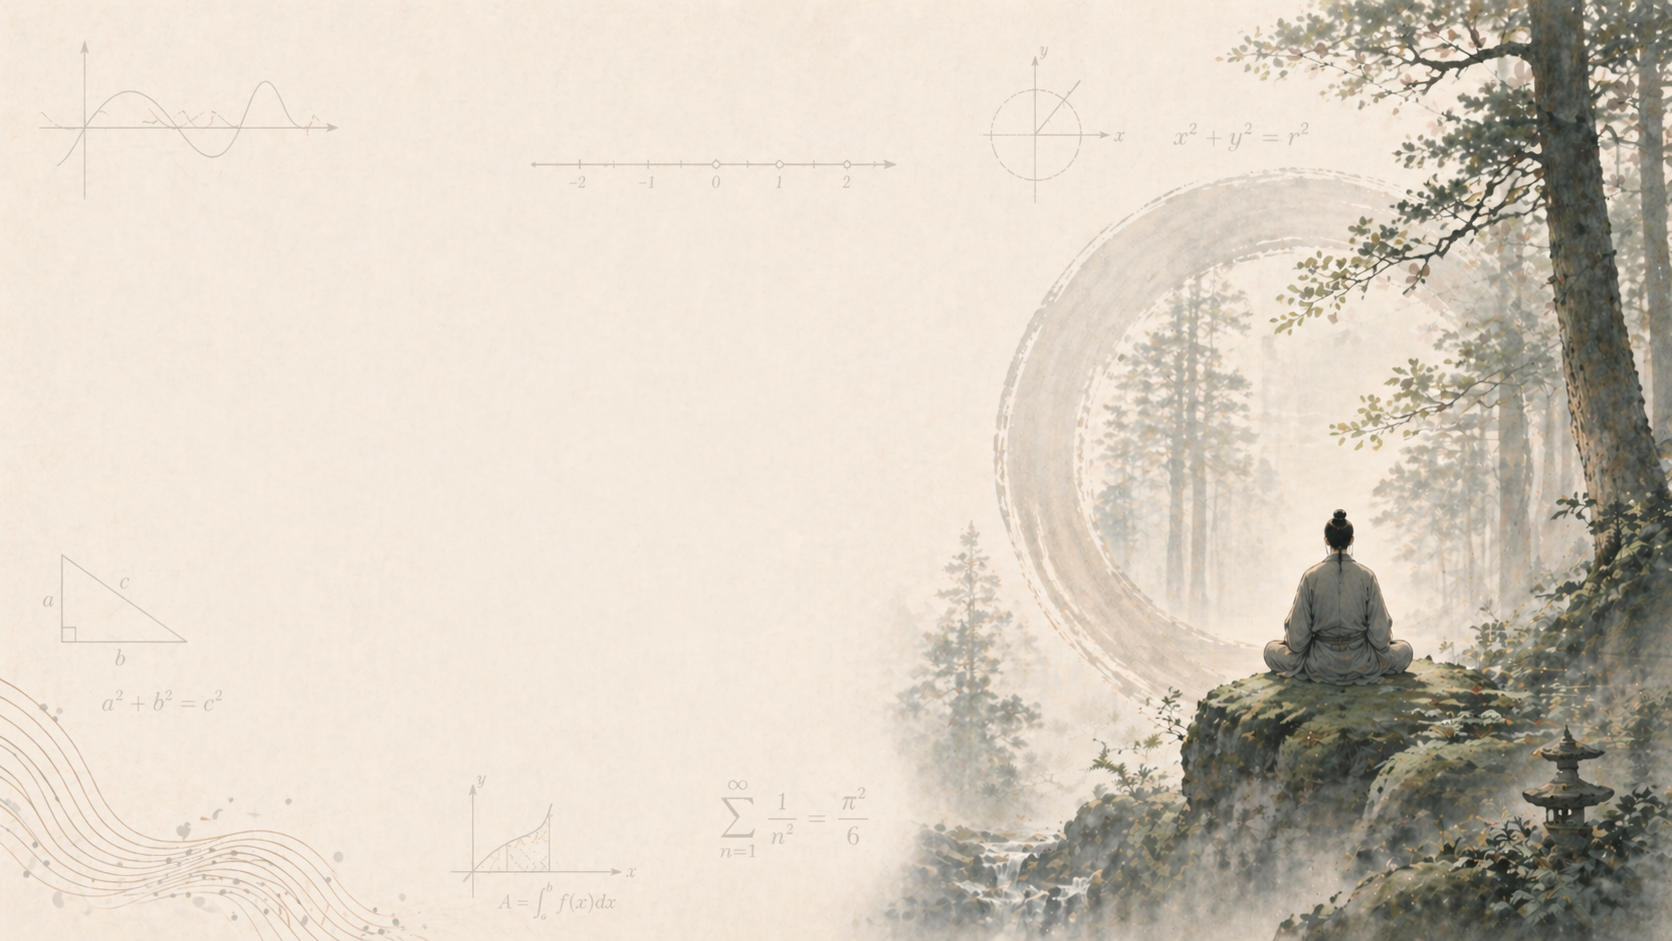
\includegraphics[width=\paperwidth,height=\paperheight,keepaspectratio=false]{chapter_03_bg_07.png}%
}
% =============================================================================
% SUMMARY
% =============================================================================
\section{Summary}

% --- Summary: Build 1/6 ---
\begin{frame}{Summary}
  \begin{hlbox}
    \textbf{Key takeaways from this section:}
    \begin{itemize}
      \item \alert{Definition 3.21:} a series $\Sigma\, a_n$ is just a
        symbol; its value is $\lim_{n} s_n$ when this limit exists
    \end{itemize}
  \end{hlbox}

  \note{
    Let us recap. Definition 3.21 is the foundation. An infinite
    series is, by definition, the limit of its sequence of partial
    sums. Convergence and divergence of the series are convergence
    and divergence of that sequence. The sum, when it exists, is a
    limit, not a finite addition.
  }
\end{frame}

% --- Summary: Build 2/6 ---
\begin{frame}{Summary}
  \begin{hlbox}
    \textbf{Key takeaways from this section:}
    \begin{itemize}
      \item \alert{Definition 3.21:} a series $\Sigma\, a_n$ is just a
        symbol; its value is $\lim_{n} s_n$ when this limit exists
      \item \alert{Theorem 3.22 (Cauchy):}
        $\Sigma\, a_n$ converges $\iff$
        $\bigl|\sum_{k=n}^{m} a_k\bigr|$ uniformly small for
        $m \geq n$ large
    \end{itemize}
  \end{hlbox}

  \note{
    Theorem 3.22 is the Cauchy criterion for series, the direct
    translation of the Cauchy criterion for sequences. A series
    converges if and only if all sufficiently far tail blocks are
    small in absolute value. This is our master tool for
    convergence proofs that do not rely on knowing the sum.
  }
\end{frame}

% --- Summary: Build 3/6 ---
\begin{frame}{Summary}
  \begin{hlbox}
    \textbf{Key takeaways from this section:}
    \begin{itemize}
      \item \alert{Definition 3.21:} a series $\Sigma\, a_n$ is just a
        symbol; its value is $\lim_{n} s_n$ when this limit exists
      \item \alert{Theorem 3.22 (Cauchy):}
        $\Sigma\, a_n$ converges $\iff$
        $\bigl|\sum_{k=n}^{m} a_k\bigr|$ uniformly small for
        $m \geq n$ large
      \item \alert{Theorem 3.23:} $\Sigma\, a_n$ converges
        $\Longrightarrow$ $a_n \to 0$
        \emph{(converse fails!)}
    \end{itemize}
  \end{hlbox}

  \note{
    Theorem 3.23 is the cheapest necessary condition. If a series
    converges, its terms tend to zero. Equivalently: if the terms
    do not tend to zero, the series cannot converge. But beware,
    the converse is false. The harmonic series, with general term
    1 over "n", has terms that obviously go to zero, yet its
    partial sums march off to infinity. Vanishing terms are
    necessary for convergence, not sufficient.
  }
\end{frame}

% --- Summary: Build 4/6 ---
\begin{frame}{Summary}
  \begin{hlbox}
    \textbf{Key takeaways from this section:}
    \begin{itemize}
      \item \alert{Definition 3.21:} a series $\Sigma\, a_n$ is just a
        symbol; its value is $\lim_{n} s_n$ when this limit exists
      \item \alert{Theorem 3.22 (Cauchy):}
        $\Sigma\, a_n$ converges $\iff$
        $\bigl|\sum_{k=n}^{m} a_k\bigr|$ uniformly small for
        $m \geq n$ large
      \item \alert{Theorem 3.23:} $\Sigma\, a_n$ converges
        $\Longrightarrow$ $a_n \to 0$
        \emph{(converse fails!)}
      \item \alert{Theorem 3.24:} if $a_n \geq 0$, convergence
        $\iff$ partial sums bounded
    \end{itemize}
  \end{hlbox}

  \note{
    Theorem 3.24 specialises to series of nonnegative real terms.
    There, the partial sums are monotonically nondecreasing, so by
    the monotone convergence theorem for sequences, convergence
    reduces to boundedness. This single observation turns
    convergence into a quantitative bound.
  }
\end{frame}

% --- Summary: Build 5/6 ---
\begin{frame}{Summary}
  \begin{hlbox}
    \textbf{Key takeaways from this section:}
    \begin{itemize}
      \item \alert{Definition 3.21:} a series $\Sigma\, a_n$ is just a
        symbol; its value is $\lim_{n} s_n$ when this limit exists
      \item \alert{Theorem 3.22 (Cauchy):}
        $\Sigma\, a_n$ converges $\iff$
        $\bigl|\sum_{k=n}^{m} a_k\bigr|$ uniformly small for
        $m \geq n$ large
      \item \alert{Theorem 3.23:} $\Sigma\, a_n$ converges
        $\Longrightarrow$ $a_n \to 0$
        \emph{(converse fails!)}
      \item \alert{Theorem 3.24:} if $a_n \geq 0$, convergence
        $\iff$ partial sums bounded
      \item \alert{Theorem 3.25 (Comparison test):} dominate by a
        known convergent / divergent series
    \end{itemize}
  \end{hlbox}

  \note{
    Theorem 3.25, the comparison test, is our first genuine
    convergence test. Bound the absolute values of your terms by
    those of a series you know converges, and convergence
    transfers. Bound a nonnegative series from below by one you
    know diverges, and divergence transfers. The whole proof is a
    one-line application of the triangle inequality and the Cauchy
    criterion.
  }
\end{frame}

% --- Summary: Build 6/6 (the slogan) ---
\begin{frame}{Summary}
  \begin{hlbox}
    \textbf{Key takeaways from this section:}
    \begin{itemize}
      \item \alert{Definition 3.21:} a series $\Sigma\, a_n$ is just a
        symbol; its value is $\lim_{n} s_n$ when this limit exists
      \item \alert{Theorem 3.22 (Cauchy):}
        $\Sigma\, a_n$ converges $\iff$
        $\bigl|\sum_{k=n}^{m} a_k\bigr|$ uniformly small for
        $m \geq n$ large
      \item \alert{Theorem 3.23:} $\Sigma\, a_n$ converges
        $\Longrightarrow$ $a_n \to 0$
        \emph{(converse fails!)}
      \item \alert{Theorem 3.24:} if $a_n \geq 0$, convergence
        $\iff$ partial sums bounded
      \item \alert{Theorem 3.25 (Comparison test):} dominate by a
        known convergent / divergent series
      \item \emph{Slogan:} \alert{a series is its sequence of
        partial sums}
    \end{itemize}
  \end{hlbox}

  \note{
    The big slogan to keep in mind, written on the last bullet, is
    that a series is its sequence of partial sums. Everything we
    proved here was really a theorem about sequences, dressed in
    series clothing. The conceptual leap is that this dressing
    matters: thinking in terms of series organises the material in
    a way that pure sequence language would not.
  }
\end{frame}

% --- Coming up next ---
\begin{frame}{Coming Up Next}
  \begin{hlbox}
    \textbf{Next section: Series of Nonnegative Terms}
    \begin{itemize}
      \item Build the \alert{reference catalogue} the comparison test
        depends on
      \item Geometric series, the harmonic series, $p$-series
      \item The Cauchy condensation test
    \end{itemize}
  \end{hlbox}

  \vspace{0.4em}
  \begin{hlbox}
    Together these turn Theorem 3.25 into a practical convergence
    test for almost everything you will meet.
  \end{hlbox}

  \note{
    Coming up next, we cash in on Theorem 3.25 by building the
    reference catalogue it depends on. We will pin down the
    geometric series, the harmonic series, and the so-called "p"
    series for various values of "p", and we will prove the Cauchy
    condensation test, which links the convergence of a series to
    that of a sparse subseries. With those reference series in
    hand, the comparison test becomes a powerful, practical
    convergence tool. See you in the next section.
  }
\end{frame}
}

\end{document}
